% https://github.com/loopspace/spath3/issues/36#issuecomment-3898385525
\documentclass[tikz,border=5pt]{standalone} 
% https://tex.stackexchange.com/a/656167/322482
\usetikzlibrary{bending,decorations.markings,arrows.meta,calc,spath3} 
\usepackage{amsmath} 
\begin{document} 
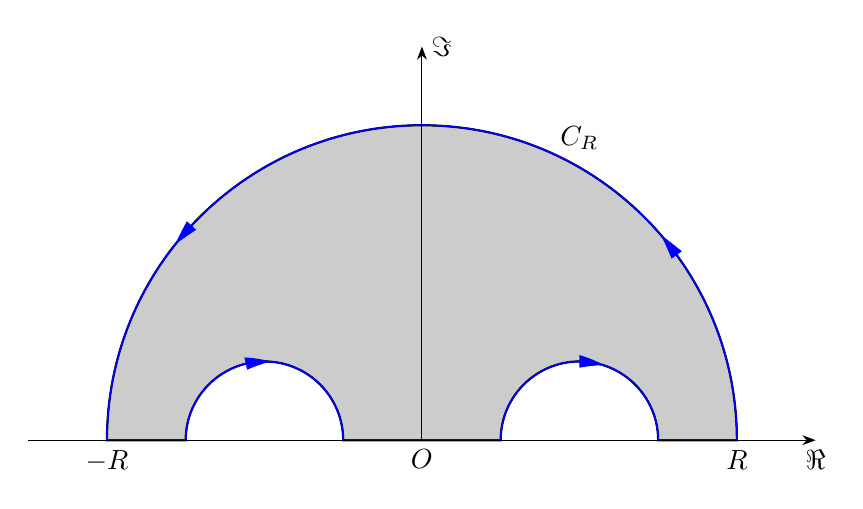
\begin{tikzpicture}[>={Kite[inset=0pt,length=.32cm,bend]}]
    \filldraw[
        thick,fill=gray!40,
        spath/save=curve,
    ]
        (4,0) node[below]{$R$} 
        arc (0:180:4) node[below]{$-R$} 
        -- (-3,0) arc(180:0:1) 
        -- (1,0) arc(180:0:1) 
        -- cycle;
    \foreach \pos in {0.05,0.175,.45,.8}{%
        \path[
            draw=blue,tips=true,->,
            spath/clone={tmp}{curve},
            spath/remove empty components={tmp},
            spath/split at keep start={tmp}{\pos},
            spath/use=tmp,
        ];
    }

    \draw[-Stealth] (-5,0) -- (5,0) node[below]{$\Re$};
    \draw[-Stealth] (0,0) -- (0,5) node[right]{$\Im$};
    \path 
        node[below] {$O$} 
        (60:4) 
        node[above=3pt] {$C_{R}$};
\end{tikzpicture}
\end{document}